\documentclass[a4paper]{book}
\usepackage{a4wide}
\usepackage{makeidx}
\usepackage{graphicx}
\usepackage{multicol}
\usepackage{float}
\usepackage{listings}
\usepackage{color}
\usepackage{textcomp}
\usepackage{alltt}
\usepackage{times}
\usepackage{ifpdf}
\ifpdf
\usepackage[pdftex,
            pagebackref=true,
            colorlinks=true,
            linkcolor=blue,
            unicode
           ]{hyperref}
\else
\usepackage[ps2pdf,
            pagebackref=true,
            colorlinks=true,
            linkcolor=blue,
            unicode
           ]{hyperref}
\usepackage{pspicture}
\fi
\usepackage[utf8]{inputenc}
\usepackage{doxygen}
\lstset{language=C++,inputencoding=utf8,basicstyle=\footnotesize,breaklines=true,breakatwhitespace=true,tabsize=8,numbers=left }
\makeindex
\setcounter{tocdepth}{3}
\renewcommand{\footrulewidth}{0.4pt}
\begin{document}
\hypersetup{pageanchor=false}
\begin{titlepage}
\vspace*{7cm}
\begin{center}
{\Large Reference Manual}\\
\vspace*{1cm}
{\large Generated by Doxygen 1.7.1}\\
\vspace*{0.5cm}
{\small Mon Nov 26 2012 13:18:04}\\
\end{center}
\end{titlepage}
\clearemptydoublepage
\pagenumbering{roman}
\tableofcontents
\clearemptydoublepage
\pagenumbering{arabic}
\hypersetup{pageanchor=true}
\chapter{Class Index}
\section{Class Hierarchy}
This inheritance list is sorted roughly, but not completely, alphabetically:\begin{DoxyCompactList}
\item \contentsline{section}{CaptureDelegate}{\pageref{classCaptureDelegate}}{}
\item \contentsline{section}{LoopThroughWithOpenGLCompositing}{\pageref{classLoopThroughWithOpenGLCompositing}}{}
\item \contentsline{section}{OpenGLComposite}{\pageref{classOpenGLComposite}}{}
\item \contentsline{section}{PinnedMemoryAllocator}{\pageref{classPinnedMemoryAllocator}}{}
\item \contentsline{section}{PlayoutDelegate}{\pageref{classPlayoutDelegate}}{}
\item \contentsline{section}{Ui\_\-LoopThroughWithOpenGLCompositingDialog}{\pageref{classUi__LoopThroughWithOpenGLCompositingDialog}}{}
\begin{DoxyCompactList}
\item \contentsline{section}{Ui::LoopThroughWithOpenGLCompositingDialog}{\pageref{classUi_1_1LoopThroughWithOpenGLCompositingDialog}}{}
\end{DoxyCompactList}
\end{DoxyCompactList}

\chapter{Class Index}
\section{Class List}
Here are the classes, structs, unions and interfaces with brief descriptions:\begin{DoxyCompactList}
\item\contentsline{section}{\hyperlink{classCaptureDelegate}{CaptureDelegate} }{\pageref{classCaptureDelegate}}{}
\item\contentsline{section}{\hyperlink{classLoopThroughWithOpenGLCompositing}{LoopThroughWithOpenGLCompositing} }{\pageref{classLoopThroughWithOpenGLCompositing}}{}
\item\contentsline{section}{\hyperlink{classUi_1_1LoopThroughWithOpenGLCompositingDialog}{Ui::LoopThroughWithOpenGLCompositingDialog} }{\pageref{classUi_1_1LoopThroughWithOpenGLCompositingDialog}}{}
\item\contentsline{section}{\hyperlink{classOpenGLComposite}{OpenGLComposite} (Les PinnedMemoryAllocators permettent une meilleure gestion de la mémoire sur les systèmes compatibles )}{\pageref{classOpenGLComposite}}{}
\item\contentsline{section}{\hyperlink{classPinnedMemoryAllocator}{PinnedMemoryAllocator} }{\pageref{classPinnedMemoryAllocator}}{}
\item\contentsline{section}{\hyperlink{classPlayoutDelegate}{PlayoutDelegate} }{\pageref{classPlayoutDelegate}}{}
\item\contentsline{section}{\hyperlink{classUi__LoopThroughWithOpenGLCompositingDialog}{Ui\_\-LoopThroughWithOpenGLCompositingDialog} }{\pageref{classUi__LoopThroughWithOpenGLCompositingDialog}}{}
\end{DoxyCompactList}

\chapter{Class Documentation}
\hypertarget{classCaptureDelegate}{
\section{CaptureDelegate Class Reference}
\label{classCaptureDelegate}\index{CaptureDelegate@{CaptureDelegate}}
}
\subsection*{Signals}
\begin{DoxyCompactItemize}
\item 
\hypertarget{classCaptureDelegate_a99141e43070b7bcee71123d1e688867f}{
void {\bfseries captureFrameArrived} (IDeckLinkVideoInputFrame $\ast$videoFrame, bool hasNoInputSource)}
\label{classCaptureDelegate_a99141e43070b7bcee71123d1e688867f}

\end{DoxyCompactItemize}
\subsection*{Public Member Functions}
\begin{DoxyCompactItemize}
\item 
\hypertarget{classCaptureDelegate_a62f27b4776e6a3621c4c7f1b8ec0a35f}{
virtual HRESULT STDMETHODCALLTYPE {\bfseries QueryInterface} (REFIID, LPVOID $\ast$)}
\label{classCaptureDelegate_a62f27b4776e6a3621c4c7f1b8ec0a35f}

\item 
\hypertarget{classCaptureDelegate_a24510dcbcfc85d855a3d6ce2ee9b0ea9}{
virtual ULONG STDMETHODCALLTYPE {\bfseries AddRef} ()}
\label{classCaptureDelegate_a24510dcbcfc85d855a3d6ce2ee9b0ea9}

\item 
\hypertarget{classCaptureDelegate_af0390f11be146651aa58e71a67d86ae3}{
virtual ULONG STDMETHODCALLTYPE {\bfseries Release} ()}
\label{classCaptureDelegate_af0390f11be146651aa58e71a67d86ae3}

\item 
\hypertarget{classCaptureDelegate_aae83bfd29866e2c41388f6e67a01220c}{
virtual HRESULT STDMETHODCALLTYPE {\bfseries VideoInputFrameArrived} (IDeckLinkVideoInputFrame $\ast$videoFrame, IDeckLinkAudioInputPacket $\ast$audioPacket)}
\label{classCaptureDelegate_aae83bfd29866e2c41388f6e67a01220c}

\item 
\hypertarget{classCaptureDelegate_a475e348f1a3aed3bee53f48f96ff2170}{
virtual HRESULT STDMETHODCALLTYPE {\bfseries VideoInputFormatChanged} (BMDVideoInputFormatChangedEvents notificationEvents, IDeckLinkDisplayMode $\ast$newDisplayMode, BMDDetectedVideoInputFormatFlags detectedSignalFlags)}
\label{classCaptureDelegate_a475e348f1a3aed3bee53f48f96ff2170}

\end{DoxyCompactItemize}


The documentation for this class was generated from the following files:\begin{DoxyCompactItemize}
\item 
OpenGLComposite.h\item 
DreamEverywhereBMD.cpp\item 
moc\_\-OpenGLComposite.cpp\end{DoxyCompactItemize}

\hypertarget{classLoopThroughWithOpenGLCompositing}{
\section{LoopThroughWithOpenGLCompositing Class Reference}
\label{classLoopThroughWithOpenGLCompositing}\index{LoopThroughWithOpenGLCompositing@{LoopThroughWithOpenGLCompositing}}
}
\subsection*{Public Member Functions}
\begin{DoxyCompactItemize}
\item 
\hyperlink{classLoopThroughWithOpenGLCompositing_afbab30002ec10d775a18a209de41e82a}{LoopThroughWithOpenGLCompositing} ()
\begin{DoxyCompactList}\small\item\em Le constructeur. \item\end{DoxyCompactList}\item 
\hypertarget{classLoopThroughWithOpenGLCompositing_a78e59cc82b757b57e29c9d87f678d017}{
\hyperlink{classLoopThroughWithOpenGLCompositing_a78e59cc82b757b57e29c9d87f678d017}{$\sim$LoopThroughWithOpenGLCompositing} ()}
\label{classLoopThroughWithOpenGLCompositing_a78e59cc82b757b57e29c9d87f678d017}

\begin{DoxyCompactList}\small\item\em Le destructeur. \item\end{DoxyCompactList}\item 
void \hyperlink{classLoopThroughWithOpenGLCompositing_a74c8a65cae511ef38b1f452ccd4285fb}{start} ()
\begin{DoxyCompactList}\small\item\em Fonction de démarrage. \item\end{DoxyCompactList}\end{DoxyCompactItemize}


\subsection{Constructor \& Destructor Documentation}
\hypertarget{classLoopThroughWithOpenGLCompositing_afbab30002ec10d775a18a209de41e82a}{
\index{LoopThroughWithOpenGLCompositing@{LoopThroughWithOpenGLCompositing}!LoopThroughWithOpenGLCompositing@{LoopThroughWithOpenGLCompositing}}
\index{LoopThroughWithOpenGLCompositing@{LoopThroughWithOpenGLCompositing}!LoopThroughWithOpenGLCompositing@{LoopThroughWithOpenGLCompositing}}
\subsubsection[{LoopThroughWithOpenGLCompositing}]{\setlength{\rightskip}{0pt plus 5cm}LoopThroughWithOpenGLCompositing::LoopThroughWithOpenGLCompositing (
\begin{DoxyParamCaption}
{}
\end{DoxyParamCaption}
)}}
\label{classLoopThroughWithOpenGLCompositing_afbab30002ec10d775a18a209de41e82a}


Le constructeur. 

\hyperlink{classLoopThroughWithOpenGLCompositing}{LoopThroughWithOpenGLCompositing} class.

Crée un \hyperlink{classOpenGLComposite}{OpenGLComposite} et l'affiche dans le QDialog

Cette classe sert de support à l'affichage du QGLWdiget d'affichage. 

\subsection{Member Function Documentation}
\hypertarget{classLoopThroughWithOpenGLCompositing_a74c8a65cae511ef38b1f452ccd4285fb}{
\index{LoopThroughWithOpenGLCompositing@{LoopThroughWithOpenGLCompositing}!start@{start}}
\index{start@{start}!LoopThroughWithOpenGLCompositing@{LoopThroughWithOpenGLCompositing}}
\subsubsection[{start}]{\setlength{\rightskip}{0pt plus 5cm}void LoopThroughWithOpenGLCompositing::start (
\begin{DoxyParamCaption}
{}
\end{DoxyParamCaption}
)}}
\label{classLoopThroughWithOpenGLCompositing_a74c8a65cae511ef38b1f452ccd4285fb}


Fonction de démarrage. 

La fonction de démarrage qui lance les entrées et sorties 

The documentation for this class was generated from the following files:\begin{DoxyCompactItemize}
\item 
LoopThroughWithOpenGLCompositing.h\item 
LoopThroughWithOpenGLCompositing.cpp\end{DoxyCompactItemize}

\hypertarget{classUi_1_1LoopThroughWithOpenGLCompositingDialog}{
\section{Ui::LoopThroughWithOpenGLCompositingDialog Class Reference}
\label{classUi_1_1LoopThroughWithOpenGLCompositingDialog}\index{Ui::LoopThroughWithOpenGLCompositingDialog@{Ui::LoopThroughWithOpenGLCompositingDialog}}
}
Inheritance diagram for Ui::LoopThroughWithOpenGLCompositingDialog:\begin{figure}[H]
\begin{center}
\leavevmode
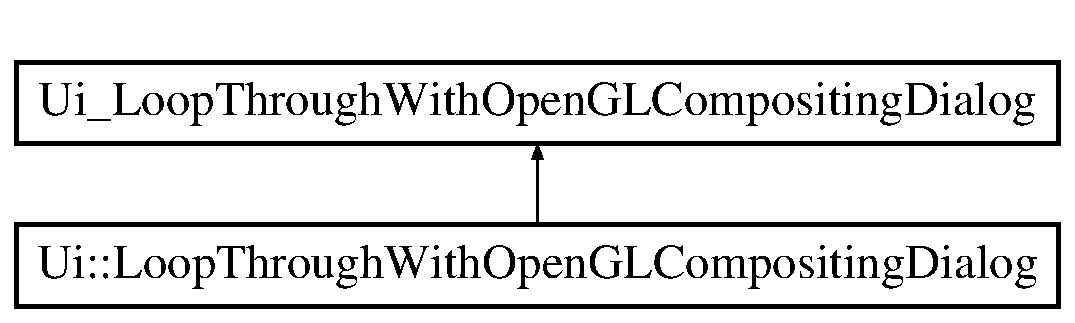
\includegraphics[height=2.000000cm]{classUi_1_1LoopThroughWithOpenGLCompositingDialog}
\end{center}
\end{figure}


The documentation for this class was generated from the following file:\begin{DoxyCompactItemize}
\item 
ui\_\-LoopThroughWithOpenGLCompositing.h\end{DoxyCompactItemize}

\hypertarget{classOpenGLComposite}{
\section{OpenGLComposite Class Reference}
\label{classOpenGLComposite}\index{OpenGLComposite@{OpenGLComposite}}
}


Les PinnedMemoryAllocators permettent une meilleure gestion de la mémoire sur les systèmes compatibles.  




{\ttfamily \#include $<$OpenGLComposite.h$>$}

\subsection*{Public Member Functions}
\begin{DoxyCompactItemize}
\item 
\hyperlink{classOpenGLComposite_a6bb5579d673170405b5ea131c454ba5c}{OpenGLComposite} (QWidget $\ast$parent=NULL)
\begin{DoxyCompactList}\small\item\em Le constructeur. \item\end{DoxyCompactList}\item 
\hyperlink{classOpenGLComposite_abe7ea6a3fbdb61a79ebde5e22929ef1a}{$\sim$OpenGLComposite} ()
\begin{DoxyCompactList}\small\item\em Le destructeur. \item\end{DoxyCompactList}\item 
bool \hyperlink{classOpenGLComposite_ab6a36e1b442176b85c26f3bab5c495a2}{InitDeckLink} ()
\begin{DoxyCompactList}\small\item\em Initialisation des cartes BMD. \item\end{DoxyCompactList}\item 
\hypertarget{classOpenGLComposite_a8d9c364bd561d2d8121d3951655dd58d}{
bool \hyperlink{classOpenGLComposite_a8d9c364bd561d2d8121d3951655dd58d}{Start} ()}
\label{classOpenGLComposite_a8d9c364bd561d2d8121d3951655dd58d}

\begin{DoxyCompactList}\small\item\em Démarrage des cartes BMD. \item\end{DoxyCompactList}\item 
\hypertarget{classOpenGLComposite_a087592bf53ea8bfe6f763bcd58da3652}{
bool \hyperlink{classOpenGLComposite_a087592bf53ea8bfe6f763bcd58da3652}{Stop} ()}
\label{classOpenGLComposite_a087592bf53ea8bfe6f763bcd58da3652}

\begin{DoxyCompactList}\small\item\em Arrêt des cartes BMD. \item\end{DoxyCompactList}\end{DoxyCompactItemize}


\subsection{Detailed Description}
Les PinnedMemoryAllocators permettent une meilleure gestion de la mémoire sur les systèmes compatibles. 

\subsection{Constructor \& Destructor Documentation}
\hypertarget{classOpenGLComposite_a6bb5579d673170405b5ea131c454ba5c}{
\index{OpenGLComposite@{OpenGLComposite}!OpenGLComposite@{OpenGLComposite}}
\index{OpenGLComposite@{OpenGLComposite}!OpenGLComposite@{OpenGLComposite}}
\subsubsection[{OpenGLComposite}]{\setlength{\rightskip}{0pt plus 5cm}OpenGLComposite::OpenGLComposite (
\begin{DoxyParamCaption}
\item[{QWidget $\ast$}]{ parent = {\ttfamily NULL}}
\end{DoxyParamCaption}
)}}
\label{classOpenGLComposite_a6bb5579d673170405b5ea131c454ba5c}


Le constructeur. 

Crée un \hyperlink{classOpenGLComposite}{OpenGLComposite} et initialise les variables, \hypertarget{classOpenGLComposite_abe7ea6a3fbdb61a79ebde5e22929ef1a}{
\index{OpenGLComposite@{OpenGLComposite}!$\sim$OpenGLComposite@{$\sim$OpenGLComposite}}
\index{$\sim$OpenGLComposite@{$\sim$OpenGLComposite}!OpenGLComposite@{OpenGLComposite}}
\subsubsection[{$\sim$OpenGLComposite}]{\setlength{\rightskip}{0pt plus 5cm}OpenGLComposite::$\sim$OpenGLComposite (
\begin{DoxyParamCaption}
{}
\end{DoxyParamCaption}
)}}
\label{classOpenGLComposite_abe7ea6a3fbdb61a79ebde5e22929ef1a}


Le destructeur. 

Détruit l'objet et appelle destruct\_\-Decklink qui détruit ce qui dépend uniquement des cartes BMD. 

\subsection{Member Function Documentation}
\hypertarget{classOpenGLComposite_ab6a36e1b442176b85c26f3bab5c495a2}{
\index{OpenGLComposite@{OpenGLComposite}!InitDeckLink@{InitDeckLink}}
\index{InitDeckLink@{InitDeckLink}!OpenGLComposite@{OpenGLComposite}}
\subsubsection[{InitDeckLink}]{\setlength{\rightskip}{0pt plus 5cm}bool OpenGLComposite::InitDeckLink (
\begin{DoxyParamCaption}
{}
\end{DoxyParamCaption}
)}}
\label{classOpenGLComposite_ab6a36e1b442176b85c26f3bab5c495a2}


Initialisation des cartes BMD. 

Réalise l'initialisation des cartes BMD en entrée/sortie Utilisera un tableau de routage 

The documentation for this class was generated from the following files:\begin{DoxyCompactItemize}
\item 
OpenGLComposite.h\item 
dessin.cpp\item 
DreamEverywhereBMD.cpp\item 
OpenGLComposite.cpp\end{DoxyCompactItemize}

\hypertarget{classPinnedMemoryAllocator}{
\section{PinnedMemoryAllocator Class Reference}
\label{classPinnedMemoryAllocator}\index{PinnedMemoryAllocator@{PinnedMemoryAllocator}}
}
\subsection*{Public Member Functions}
\begin{DoxyCompactItemize}
\item 
\hypertarget{classPinnedMemoryAllocator_aad2d856c8c144dca3c2274dbbc955748}{
{\bfseries PinnedMemoryAllocator} (QGLWidget $\ast$context, const char $\ast$name, unsigned cacheSize)}
\label{classPinnedMemoryAllocator_aad2d856c8c144dca3c2274dbbc955748}

\item 
\hypertarget{classPinnedMemoryAllocator_a7fbcbdfcc5a9c1a9c8cdd9c9bd018db4}{
GLuint {\bfseries bufferObjectForPinnedAddress} (int bufferSize, const void $\ast$address)}
\label{classPinnedMemoryAllocator_a7fbcbdfcc5a9c1a9c8cdd9c9bd018db4}

\item 
\hypertarget{classPinnedMemoryAllocator_a989b461a86bc64a045627276520908c4}{
void {\bfseries unPinAddress} (const void $\ast$address)}
\label{classPinnedMemoryAllocator_a989b461a86bc64a045627276520908c4}

\item 
\hypertarget{classPinnedMemoryAllocator_a8994f08854a3c20c183285a11185edce}{
virtual HRESULT STDMETHODCALLTYPE {\bfseries QueryInterface} (REFIID iid, LPVOID $\ast$ppv)}
\label{classPinnedMemoryAllocator_a8994f08854a3c20c183285a11185edce}

\item 
\hypertarget{classPinnedMemoryAllocator_ad64b742fa613fd34992b740a84b174e1}{
virtual ULONG STDMETHODCALLTYPE {\bfseries AddRef} (void)}
\label{classPinnedMemoryAllocator_ad64b742fa613fd34992b740a84b174e1}

\item 
\hypertarget{classPinnedMemoryAllocator_abf0039df0bd78b1a18ce310ac4f3c089}{
virtual ULONG STDMETHODCALLTYPE {\bfseries Release} (void)}
\label{classPinnedMemoryAllocator_abf0039df0bd78b1a18ce310ac4f3c089}

\item 
\hypertarget{classPinnedMemoryAllocator_a9de61e0e5eaa71e0c2987d9f26209e08}{
virtual HRESULT STDMETHODCALLTYPE {\bfseries AllocateBuffer} (uint32\_\-t bufferSize, void $\ast$$\ast$allocatedBuffer)}
\label{classPinnedMemoryAllocator_a9de61e0e5eaa71e0c2987d9f26209e08}

\item 
\hypertarget{classPinnedMemoryAllocator_a51521a04d32cc011d7bfb1e639521ef8}{
virtual HRESULT STDMETHODCALLTYPE {\bfseries ReleaseBuffer} (void $\ast$buffer)}
\label{classPinnedMemoryAllocator_a51521a04d32cc011d7bfb1e639521ef8}

\item 
\hypertarget{classPinnedMemoryAllocator_a536f2c73de3a20f61fe577c29ac067f6}{
virtual HRESULT STDMETHODCALLTYPE {\bfseries Commit} ()}
\label{classPinnedMemoryAllocator_a536f2c73de3a20f61fe577c29ac067f6}

\item 
\hypertarget{classPinnedMemoryAllocator_a11d0bf5a7d689293d3f2bdeb7ad980b2}{
virtual HRESULT STDMETHODCALLTYPE {\bfseries Decommit} ()}
\label{classPinnedMemoryAllocator_a11d0bf5a7d689293d3f2bdeb7ad980b2}

\end{DoxyCompactItemize}


The documentation for this class was generated from the following files:\begin{DoxyCompactItemize}
\item 
OpenGLComposite.h\item 
pinnedmemoryallocator.cpp\end{DoxyCompactItemize}

\hypertarget{classPlayoutDelegate}{
\section{PlayoutDelegate Class Reference}
\label{classPlayoutDelegate}\index{PlayoutDelegate@{PlayoutDelegate}}
}
\subsection*{Signals}
\begin{DoxyCompactItemize}
\item 
\hypertarget{classPlayoutDelegate_a332c5736a79fdc8222fc28d7028b83de}{
void {\bfseries playoutFrameCompleted} (IDeckLinkVideoFrame $\ast$completedFrame, BMDOutputFrameCompletionResult result)}
\label{classPlayoutDelegate_a332c5736a79fdc8222fc28d7028b83de}

\end{DoxyCompactItemize}
\subsection*{Public Member Functions}
\begin{DoxyCompactItemize}
\item 
\hypertarget{classPlayoutDelegate_a7414655cf0e673b37825cd97f187388a}{
virtual HRESULT STDMETHODCALLTYPE {\bfseries QueryInterface} (REFIID, LPVOID $\ast$)}
\label{classPlayoutDelegate_a7414655cf0e673b37825cd97f187388a}

\item 
\hypertarget{classPlayoutDelegate_af175bef8fab8330f8469295fb68fd0ea}{
virtual ULONG STDMETHODCALLTYPE {\bfseries AddRef} ()}
\label{classPlayoutDelegate_af175bef8fab8330f8469295fb68fd0ea}

\item 
\hypertarget{classPlayoutDelegate_a835091532e89964d47baa9012f6aca33}{
virtual ULONG STDMETHODCALLTYPE {\bfseries Release} ()}
\label{classPlayoutDelegate_a835091532e89964d47baa9012f6aca33}

\item 
\hypertarget{classPlayoutDelegate_abe39d5f30e540ca8b14bda5c74ed8110}{
virtual HRESULT STDMETHODCALLTYPE {\bfseries ScheduledFrameCompleted} (IDeckLinkVideoFrame $\ast$completedFrame, BMDOutputFrameCompletionResult result)}
\label{classPlayoutDelegate_abe39d5f30e540ca8b14bda5c74ed8110}

\item 
\hypertarget{classPlayoutDelegate_a6f604d26f72c6f01d1dd5a7eb84dbd78}{
virtual HRESULT STDMETHODCALLTYPE {\bfseries ScheduledPlaybackHasStopped} ()}
\label{classPlayoutDelegate_a6f604d26f72c6f01d1dd5a7eb84dbd78}

\end{DoxyCompactItemize}


The documentation for this class was generated from the following files:\begin{DoxyCompactItemize}
\item 
OpenGLComposite.h\item 
DreamEverywhereBMD.cpp\item 
moc\_\-OpenGLComposite.cpp\end{DoxyCompactItemize}

\hypertarget{classUi__LoopThroughWithOpenGLCompositingDialog}{
\section{Ui\_\-LoopThroughWithOpenGLCompositingDialog Class Reference}
\label{classUi__LoopThroughWithOpenGLCompositingDialog}\index{Ui\_\-LoopThroughWithOpenGLCompositingDialog@{Ui\_\-LoopThroughWithOpenGLCompositingDialog}}
}
Inheritance diagram for Ui\_\-LoopThroughWithOpenGLCompositingDialog:\begin{figure}[H]
\begin{center}
\leavevmode
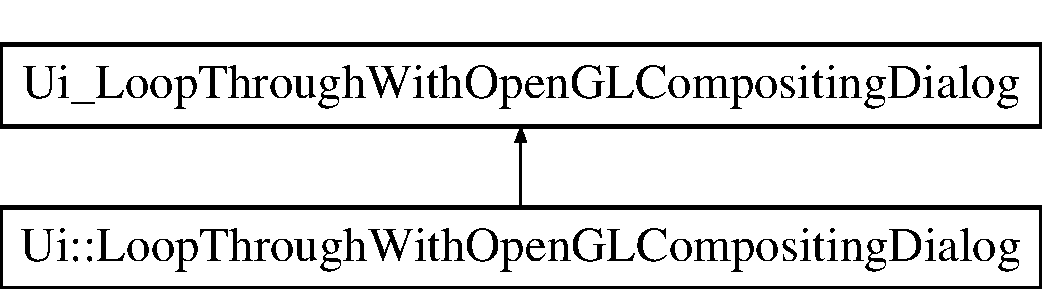
\includegraphics[height=2.000000cm]{classUi__LoopThroughWithOpenGLCompositingDialog}
\end{center}
\end{figure}
\subsection*{Public Member Functions}
\begin{DoxyCompactItemize}
\item 
\hypertarget{classUi__LoopThroughWithOpenGLCompositingDialog_a1d92e6b1a53ddc238314b693d0a9454a}{
void {\bfseries setupUi} (QDialog $\ast$LoopThroughWithOpenGLCompositingDialog)}
\label{classUi__LoopThroughWithOpenGLCompositingDialog_a1d92e6b1a53ddc238314b693d0a9454a}

\item 
\hypertarget{classUi__LoopThroughWithOpenGLCompositingDialog_a9310c5d62a2151eadec44bee103cf58c}{
void {\bfseries retranslateUi} (QDialog $\ast$LoopThroughWithOpenGLCompositingDialog)}
\label{classUi__LoopThroughWithOpenGLCompositingDialog_a9310c5d62a2151eadec44bee103cf58c}

\end{DoxyCompactItemize}
\subsection*{Public Attributes}
\begin{DoxyCompactItemize}
\item 
\hypertarget{classUi__LoopThroughWithOpenGLCompositingDialog_a08323b4d0e4837e5ba449a9d33d10b0e}{
QVBoxLayout $\ast$ {\bfseries verticalLayout}}
\label{classUi__LoopThroughWithOpenGLCompositingDialog_a08323b4d0e4837e5ba449a9d33d10b0e}

\end{DoxyCompactItemize}


The documentation for this class was generated from the following file:\begin{DoxyCompactItemize}
\item 
ui\_\-LoopThroughWithOpenGLCompositing.h\end{DoxyCompactItemize}

\printindex
\end{document}
